% -*- TeX:SI -*-
% slovene sub-mode for spell check

\documentclass[a4paper,twoside,openright,12pt]{book}
\usepackage[cp1250]{inputenc}  %Kodna stran za Windows okolje, za linux je kodna stran latin2
\usepackage[Slovene]{babel}    % pravila za slovensko deljenje besed
\usepackage[pdftex]{UNI-LJ-FE-Diploma} %Stil za diplome na Fakulteti za elektrotehniko (za pdfTeX v MkiTex)
%\usepackage[pctex]{UNI-LJ-FE-Diploma} %Stil za diplome na Fakulteti za elektrotehniko  (za pcTex)

%*************************** PRILAGODITVE *****************************
% mapa s slikami
\potgrafike{./Slike/}
%prilagoditev levega roba sodih strani. �e se pri dvostranskem tisku robovi ne umemajo se lahko pove�a ali pomanj�a
\zamaknirobsodihstrani{0mm}

%*************************** NASLOVNA STRAN *****************************
\naslov{Vodenje robota v stiku s podajnim objektom}
\avtor{Timotej Ga�par} \univerza{Univerza v Ljubljani}
\fakulteta{Fakulteta za elektrotehniko}
\delo{Magistrsko delo}
\date{Ljubljana, 2015}
\mentor{prof. dr. Ime Priimek}
%\somentor{prof. dr. Ime Priimek}
\begin{document}

%------------------------ ZA�ETNI DEL -----------------------------------
\frontmatter
%------------------------------------------------------------------------


%************************ NASLOVNA STRAN ********************************
\maketitle


%*************************** ZAHVALA ************************************
\zahvala V zahvali se kandidati zahvali mentorju in poimensko tudi
vsem sodelavcem in prijateljem, ki so pomagali in prispevali pri
delu v laboratoriju, na ra�unalniku, v delavnici, pri tehni�ni
izdelavi dela in drugje.


%*************************** VSEBINA *************************************
\tableofcontents

%*************************** SEZNAM SLIK in TABEL  ***********************
\seznamslik
\seznamtabel

%***************************  SEZNAM UPORABLJENIH SIMBOLOV  **************

\seznamsimbolov

V pri�ujo�em zaklju�nem delu so uporabljeni naslednje veli�ine in
simboli:

\begin{table}[h]
\centering
%\begin{footnotesize}
\begin{tabular}{l l l l}
 \hline \multicolumn{2}{c}{\bf{Veli�ina / oznaka}} & \multicolumn{2}{c}{\bf{Enota}}  \\
 \hline
Ime & Simbol & Ime & Simbol \\
 \hline
 �as & $t$  & sekunda & s \\
 frekvenca & $f$  & Hertz & Hz \\
 tlak & $p$  & Pascal & Pa \\
 sila vzgona & $\textbf{\textit{f}}_\text{vz}$  & Newton & N \\
 gostota & $\rho$  & - & kg/m$^3$ \\
 masa telesa  & $m_\text{t}$  & kilogram & kg \\
 vhodna napestost & $U_\text{vh}$ & volt  & V \\
 Jacobijeva matrika & $\mathbf{J}$  & - & - \\
  \hline
\end{tabular}
%\end{footnotesize}
  \caption{Veli�ine in simboli}
  \label{prebojne_trdnosti}
\end{table}

Pri �emer so vektorji in matrike napisani s poudarjeno pisavo.
Natan�nej�i pomen simbolov in njihovih indeksov je razviden iz
ustreznih slik ali pa je pojasnjen v spremljajo�em besedilu, kjer je
simbol uporabljen.


%------------------------ GLAVNI DEL ------------------------------------
\mainmatter
%-------------------------------------------------------------------------


%********************* POVZETEK V SLOVEN��INI ****************************
\povzetek

\kljucnebesede beseda1, beseda2, beseda3


%*************************** POVZETEK V ANGLE��INI ***********************
\abstract

The thesis addresses ...

\keywords word1, word2, word3


%***************************** UVOD **************************************
\chapter{Uvod} \label{uvod}


\cite{miklavvcivc2010objavljanje} ali \cite[stran 520 -
534]{juvznivc1992diplomska}.

%*********************** OSREDNJA POGLAVJA ********************************
\chapter{Izbira teme zaklju�nega dela} \label{izbira_teme}

\begin{enumerate}

\item 
\end{enumerate}

\chapter{Prijava zaklju�nega dela} \label{prijava}

\begin{enumerate}
\item 
\end{enumerate}

\chapter{Navodilo za pisanje} \label{navodilo_pisanje}

\section{Splo�na navodila} \label{splosna_navodila}

\begin{enumerate}
\item 
\end{enumerate}

\section{Podrobna navodila} \label{podrobna_navodila}

\subsection{Primer pisanja ena�b} \label{vnos_enacb}

\subsection{Slike} \label{vnos_slik}





\slikaeps{Primer vklju�itve slike}{vektorska_slika_1}

%namesto makroja \slikaeps se v MikTexu uporabi tudi naslednji na�in. Za preizkus odkomentirajte spodnje vrstice. Ne dela v PcTeXu.
%\begin{figure}[h]
%\centering
%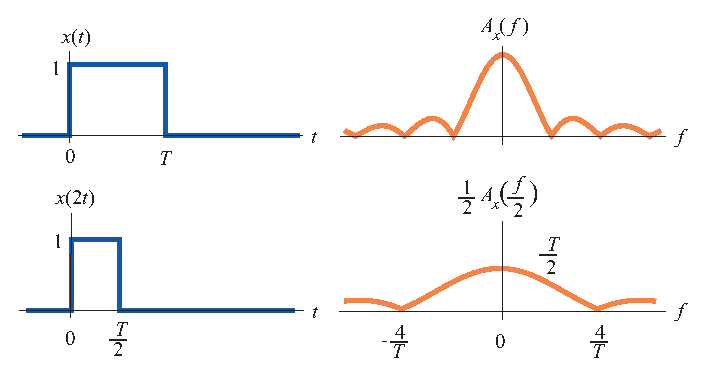
\includegraphics[width=0.75\columnwidth]{vektorska_slika_1.eps}
%\caption{\label{oblika_signalov} Primer vklju�itve slike}
%\end{figure}


\subsection{Tabele}


\begin{table}[h]
\centering
\begin{footnotesize}
\begin{tabular}{|l||c|c|}
 \hline Izolant (pri $20^o$C) & $\emph{E}_p$ / (V/m) & $U /$ V  \\
 \hline \hline
 zrak & 3  & 30 \\
 trd papir &  10 & 40 \\
 trda guma & 10  & 36 \\
  transformatorsko olje & 15 & 34.5 \\
   porcelan & 20 & 45 \\
   polivinilklorid (PVC) & 50 & 70 \\
    polistirol & 80  & 45\\
  \hline
\end{tabular}
\end{footnotesize}
  \caption{Prebojne trdnosti izolantov in priklju�ne napetosti}
  \label{prebojne_trdnosti}
\end{table}

\subsection{Programska koda}

Manj�i deli programske kode so lahko navedeni in opisani v tekstu.
Oblika teksta programske kode se lo�i od oblike ostalega teksta.
Primer:

Funkcija, ki omogo�a prenos podatkov, je naslednja:

\small
\begin{verbatim}
void I2C_Transfer(unsigned Addr,unsigned Data) {
    I2CAddress = Addr;
    I2CData = Data;

    I2CONCLR = 0x000000FF;  // Izbris I2C nastavitev
    I2CONSET = 0x00000040;  // Vklop I2C prenosa
    I2CONSET = 0x00000020;  // Start signal
}
\end{verbatim}
\normalsize


\chapter{Oddaja zaklju�nega dela} \label{oddaja}



\chapter{Zagovor zaklju�nega dela} \label{zagovor}

\chapter{Zaklju�ek} \label{zakljucek}


%**************** LITERATURA ************************
\bibliographystyle{ieeetrslo}
\bibliography{literatura}

%**************** PRILOGE ************************


\appendix
\chapter{Urejanje dokumentov z orodjem LaTex} \label{dodatekA}


Postopek dela:
\begin{description}

\end{description}

\chapter{Primer LaTex kode} \label{dodatekB}

\chapter{Vklju�evanje slik v okolju LaTex} \label{dodatekC}

\chapter{Instalacija programskih orodij za urejanje teksta v
okolju LaTex } \label{dodatekD}

\chapter{Predloge za navajanje literature - baza BibTex}
\label{dodatekE}

\footnotesize
\begin{verbatim}
@ARTICLE{clanek1,
   author = "L[eslie] A. Aamport",
   title = "The Gnats and Gnus Document Preparation System",
   journal = "\mbox{G-Animal's} Journal",
   year = 1986,
   volume = 41,
   number = 7,
   pages = "73-77",
   month = jul,
}

@BOOK{knjiga1,
   author = "Donald E. Knuth",
   title = "Seminumerical Algorithms",
   publisher = "Addison-Wesley",
   address = "Reading, Massachusetts",
   year = "1981",
}


@INPROCEEDINGS{vzborniku,
   author = "Alfred V. Oaho and Jeffrey D. Ullman and Mihalis Yannakakis",
   title = "On Notions of Information Transfer in {VLSI} Circuits",
   editor = "Wizard V. Oz and Mihalis Yannakakis",
   booktitle = "Proc. Fifteenth Annual ACM" # STOC,
   pages = "133--139",
   month = mar,
   year = 1983,
   address = "Boston",
   publisher = "Academic Press",
}


@misc{spletna_stran,
  author = "LLC",
  title = "{MS Windows NT Kernel Description [Online]}",
  howpublished = "Dosegljivo: \url{http://web.archive.org}",
  note = "[Dostopano: 19. 4. 2013]"
}
\end{verbatim}
\normalsize



\end{document}
